\documentclass[aspectratio=169,10pt]{beamer}
\usetheme{metropolis}
\usepackage{amsmath,amssymb,bm}
\usepackage{siunitx}
\usepackage{booktabs}
\usepackage{tikz}
\usetikzlibrary{arrows.meta,calc,positioning}
\usepackage{pgfplots}
\pgfplotsset{compat=1.17}
\sisetup{per-mode=symbol,detect-all}
\metroset{numbering=fraction,progressbar=frametitle,block=fill}
\tikzset{capt/.style={text width=5.2cm,align=center}}
\hypersetup{colorlinks=true,urlcolor=blue!60!black,linkcolor=.}
% ITU logo on every frame (top-right): white version on the dark title bar, navy on the title page.
\addtobeamertemplate{frametitle}{}{%
  \begin{tikzpicture}[remember picture,overlay]
    \node[anchor=north east,yshift=-1.5pt,xshift=-6pt] at (current page.north east) {
\includegraphics[height=0.7cm]{logos/itu_logo_beyaz.pdf}};
  \end{tikzpicture}}
\titlegraphic{\hfill
\includegraphics[height=1.6cm]{logos/itu_logo_laci.pdf}}

\title{Lecture 2: Fatigue --- Stress-Life and Strain-Life}
\subtitle{UCK 364E Design of Machine Elements}
\author{Prof.\ Dr.\ Onur Tunçer}
\institute{Department of Aeronautical Engineering, Istanbul Technical University}
\date{Fall 2026}

\begin{document}
\maketitle

\begin{frame}{Today}
\begin{enumerate}
  \item Why fatigue, not static strength, sizes an aircraft
  \item The three stages of damage and how to read a fracture surface
  \item Describing a cycle: $\sigma_a$, $\sigma_m$, $R$, $\Delta\sigma$
  \item S--N curves, the endurance limit, and why aluminium has none
  \item From specimen to component: the Marin factors
  \item Notches: $K_t\to K_f$ and notch sensitivity
  \item Mean stress: Goodman, Gerber, Soderberg, Morrow
  \item Variable amplitude: Miner's rule and rainflow counting
  \item Strain-life: Coffin--Manson and Neuber's rule
  \item Safe-life, fail-safe, damage tolerance --- and the scatter factor
\end{enumerate}
\end{frame}

\section{Why fatigue governs}

\begin{frame}{Last time every margin was huge}
\begin{itemize}
  \item Fuselage skin: $\mathrm{MS}_{\text{ult}}=2.86$
  \item Wing lug in bearing: $\mathrm{MS}_{\text{ult}}=0.70$
  \item Actuator rod end: $\mathrm{MS}_{\text{y}}=5.6$
\end{itemize}
\vspace{4pt}
Nothing on an aircraft is sized by \emph{one} application of load. What sizes it is \alert{repetition} far below the static allowable:
\begin{columns}[T]
\column{0.5\textwidth}
\begin{itemize}
  \item 1 pressurisation cycle per flight
  \item 1 landing impact per flight
\end{itemize}
\column{0.5\textwidth}
\begin{itemize}
  \item gusts, every hour of cruise
  \item propeller / rotor vibration at 10--1000\,Hz
\end{itemize}
\end{columns}
\begin{alertblock}{The central fact}
A metal loaded repeatedly well below yield will eventually crack. No static margin protects you. Only: lower cyclic stress, fewer cycles, or find the crack first.
\end{alertblock}
\end{frame}

\begin{frame}{Three stages of fatigue damage}
\footnotesize
\begin{columns}[T]
\column{0.56\textwidth}
\begin{enumerate}
  \item \alert{Initiation} --- cyclic slip, intrusions and extrusions, a microcrack one grain across. At a \emph{free surface}, at a \emph{stress concentration}. Up to 90\% of life in a polished specimen; almost none in a notched or corroded part.
  \item \alert{Stable growth} --- one striation per cycle; beach marks record load changes. Described by fracture mechanics (next lecture).
  \item \alert{Final fracture} --- the remaining section fails statically, in one cycle.
\end{enumerate}
\column{0.44\textwidth}
\centering
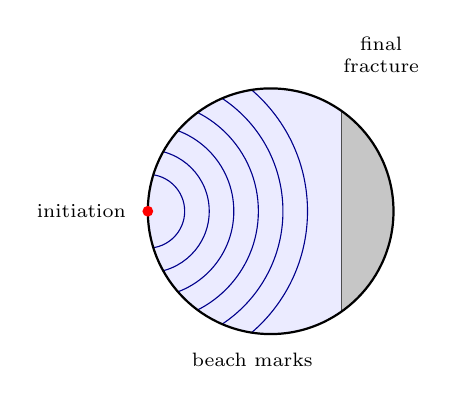
\begin{tikzpicture}[scale=0.78,>=Stealth,font=\scriptsize]
\coordinate (I) at (-2.0,0);
\begin{scope}
  \clip (0,0) circle (2.0);
  \fill[blue!8] (-2.2,-2.2) rectangle (2.2,2.2);
  \foreach \r in {0.6,1.0,1.4,1.8,2.2,2.6} \draw[blue!55!black] (I) circle (\r);
  \fill[gray!45] (1.15,-2.2) rectangle (2.3,2.2);
  \draw[gray!60!black] (1.15,-2.2) -- (1.15,2.2);
\end{scope}
\draw[thick] (0,0) circle (2.0);
\fill[red] (I) circle (2.5pt);
\node[anchor=east,align=right] at (-2.2,0) {initiation};
\node[anchor=north] at (-0.3,-2.15) {beach marks};
\node[anchor=south,align=center] at (1.8,2.1) {final\\ fracture};
\end{tikzpicture}
\end{columns}
\end{frame}


\begin{frame}{How a crack is born: slip, intrusions, extrusions}
\centering

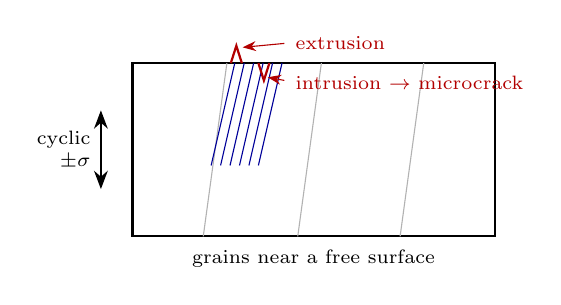
\begin{tikzpicture}[scale=1.0,>=Stealth,font=\scriptsize]
% grains
\draw[thick] (0,0) rectangle (4.6,2.2);
\foreach \x/\y in {0.9/0,2.1/0,3.4/0} \draw[gray!60] (\x,0) -- ($(\x,0)+(0.3,2.2)$);
\node[anchor=north] at (2.3,-0.05) {grains near a free surface};
% slip bands in one grain
\foreach \i in {0,...,5} \draw[blue!60!black] ({1.3+\i*0.12},2.2) -- ({1.0+\i*0.12},0.9);
% extrusion / intrusion on the surface
\draw[thick,red!70!black] (1.25,2.2) -- (1.32,2.42) -- (1.39,2.2);
\draw[thick,red!70!black] (1.60,2.2) -- (1.67,1.98) -- (1.74,2.2);
\node[anchor=west,red!70!black] at (1.95,2.45) {extrusion};
\node[anchor=west,red!70!black] at (1.95,1.95) {intrusion $\rightarrow$ microcrack};
\draw[->,red!70!black] (1.93,2.45) -- (1.40,2.40);
\draw[->,red!70!black] (1.93,1.98) -- (1.72,2.02);
\draw[<->,thick] (-0.4,0.6) -- (-0.4,1.6) node[midway,left,align=right] {cyclic\\ $\pm\sigma$};
\end{tikzpicture}

\vspace{4pt}
\footnotesize
Cyclic slip in favourably oriented \emph{surface} grains is irreversible: each cycle leaves a step. Steps pile up into an extrusion and its matching intrusion --- a notch one grain deep that the next cycles turn into a microcrack. This is why fatigue is a surface phenomenon, and why surface finish, peening and corrosion matter more than anything else you can change.
\end{frame}

\begin{frame}{The life of a crack at a fastener hole}
\centering

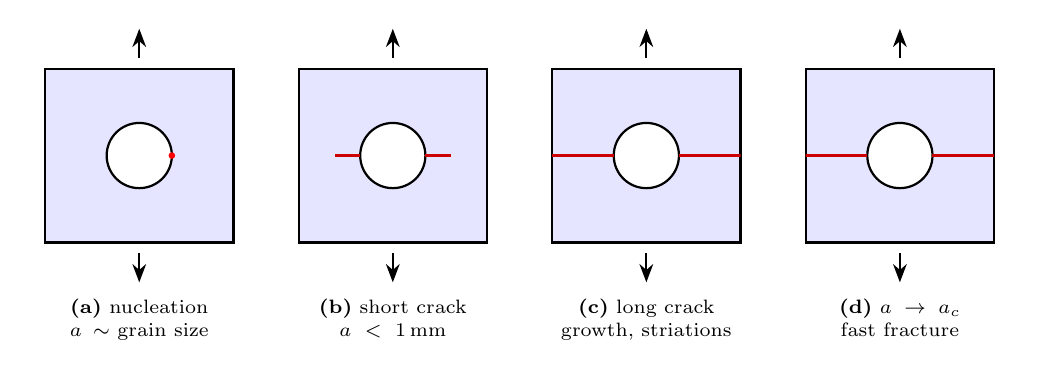
\begin{tikzpicture}[scale=0.92,>=Stealth,font=\scriptsize]
\foreach \i/\a/\lab in {0/0.0/{\textbf{(a)} nucleation\\ $a\sim$ grain size}, 1/0.35/{\textbf{(b)} short crack\\ $a<\SI{1}{mm}$}, 2/0.9/{\textbf{(c)} long crack\\ growth, striations}, 3/1.25/{\textbf{(d)} $a\to a_c$\\ fast fracture}} {
  \begin{scope}[xshift={\i*3.5cm}]
    \fill[blue!10] (0,0) rectangle (2.6,2.4);
    \draw[thick] (0,0) rectangle (2.6,2.4);
    \fill[white] (1.3,1.2) circle (0.45);
    \draw[thick] (1.3,1.2) circle (0.45);
    \begin{scope}\clip (0,0) rectangle (2.6,2.4);
    \ifnum\i>0
      \draw[red!80!black,line width=1.1pt] (1.75,1.2) -- ({1.75+\a},1.2);
      \draw[red!80!black,line width=1.1pt] (0.85,1.2) -- ({0.85-\a},1.2);
    \else
      \fill[red] (1.75,1.2) circle (1.3pt);
    \fi
    \end{scope}
    \draw[->,thick] (1.3,2.55) -- (1.3,2.95); \draw[->,thick] (1.3,-0.15) -- (1.3,-0.55);
    \node[anchor=north,align=center,text width=2.6cm] at (1.3,-0.65) {\lab};
  \end{scope}
}
\end{tikzpicture}

\vspace{6pt}
\footnotesize
(a) and (b) are \alert{initiation} --- the S--N and $\varepsilon$--N methods of this lecture predict the cycles spent here. (c) and (d) are \alert{crack growth} --- fracture mechanics, next lecture. Note that nothing visible happens until late in the life.
\end{frame}

\begin{frame}{Crack length against cycles: why inspection intervals exist}
\centering

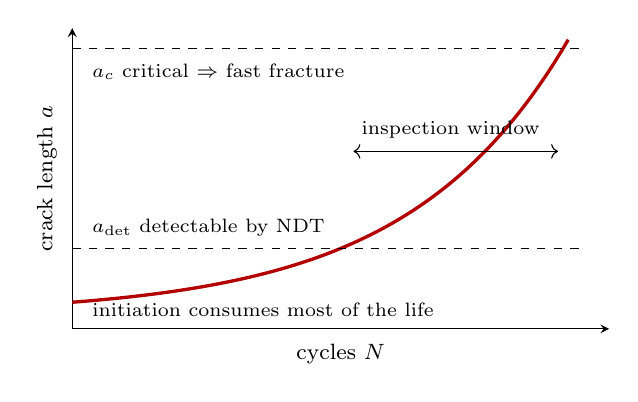
\begin{tikzpicture}
\begin{axis}[width=8.4cm,height=5.4cm,xlabel={cycles $N$},ylabel={crack length $a$},
 xmin=0,xmax=1.05,ymin=0,ymax=1.05,xtick=\empty,ytick=\empty,axis lines=left,
 label style={font=\footnotesize}]
\addplot[very thick,red!70!black,domain=0:0.97,samples=200]{0.05+0.06*exp(3.2*x)/exp(3.2*0.97)*16};
\draw[dashed] (axis cs:0,0.98) -- (axis cs:1.0,0.98);
\node[font=\scriptsize,anchor=north west] at (axis cs:0.02,0.96) {$a_c$ critical $\Rightarrow$ fast fracture};
\draw[dashed] (axis cs:0,0.28) -- (axis cs:1.0,0.28);
\node[font=\scriptsize,anchor=south west] at (axis cs:0.02,0.29) {$a_{\text{det}}$ detectable by NDT};
\draw[<->] (axis cs:0.55,0.62) -- (axis cs:0.95,0.62); \node[font=\scriptsize,anchor=south] at (axis cs:0.74,0.63) {inspection window};
\node[font=\scriptsize,anchor=south west] at (axis cs:0.02,0.01) {initiation consumes most of the life};
\end{axis}
\end{tikzpicture}

\vspace{-2pt}
\begin{columns}[T]
\column{0.5\textwidth}\footnotesize
\begin{itemize}
  \item Growth is \alert{accelerating}: the longer the crack, the faster it grows
  \item Most of the life is spent at a size nobody can see
\end{itemize}
\column{0.5\textwidth}\footnotesize
\begin{itemize}
  \item The usable window runs from $a_{\text{det}}$ (what NDT can find) to $a_c$ (fast fracture)
  \item Inspections must fit \alert{at least twice} inside that window
\end{itemize}
\end{columns}
\end{frame}

\begin{frame}{Reading the fracture surface: beach marks and striations}
\centering

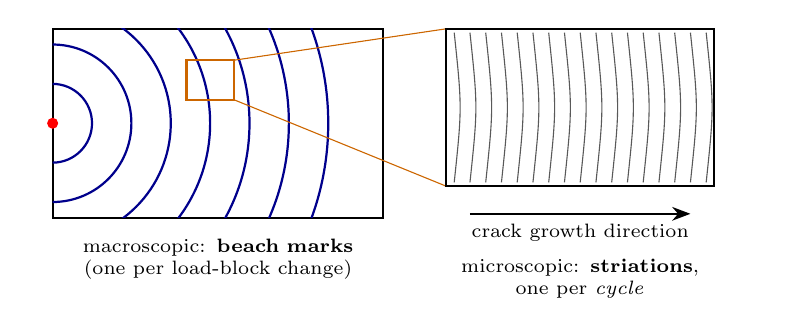
\begin{tikzpicture}[scale=1.0,>=Stealth,font=\scriptsize]
% macro beach marks
\draw[thick] (0,0) rectangle (4.2,2.4);
\coordinate (O) at (0,1.2);
\begin{scope}\clip (0,0) rectangle (4.2,2.4);
 \foreach \r in {0.5,1.0,1.5,2.0,2.5,3.0,3.5} \draw[blue!55!black,thick] (O) circle (\r);
\end{scope}
\fill[red] (O) circle (2pt);
\node[anchor=north,align=center,text width=4.6cm] at (2.1,-0.15) {macroscopic: \textbf{beach marks}\\ (one per load-block change)};
% zoom box
\draw[orange!80!black,thick] (1.7,1.5) rectangle (2.3,2.0);
\draw[orange!80!black] (2.3,2.0) -- (5.0,2.4); \draw[orange!80!black] (2.3,1.5) -- (5.0,0.4);
\begin{scope}[xshift=5.0cm,yshift=0.4cm]
 \draw[thick] (0,0) rectangle (3.4,2.0);
 \foreach \i in {0,...,16} \draw[gray!70!black] ({0.1+\i*0.2},0.05) .. controls ({0.2+\i*0.2},1.0) .. ({0.1+\i*0.2},1.95);
 \draw[->,thick] (0.3,-0.35) -- (3.1,-0.35) node[midway,below] {crack growth direction};
 \node[anchor=north,align=center,text width=4.6cm] at (1.7,-0.8) {microscopic: \textbf{striations},\\ one per \emph{cycle}};
\end{scope}
\end{tikzpicture}

\vspace{4pt}
\footnotesize
Beach marks are visible to the eye and mark changes of load \emph{block} (a flight, a shutdown). Striations need an electron microscope and mark individual \emph{cycles}. Counting back from the striation spacing is how an investigator reconstructs how long a crack had been growing.
\end{frame}

\section{Describing a cycle}

\begin{frame}{The language of a cycle}
\footnotesize
\begin{columns}[T]
\column{0.45\textwidth}
\begin{align*}
\sigma_m&=\tfrac12(\sigma_{\max}+\sigma_{\min})\\
\sigma_a&=\tfrac12(\sigma_{\max}-\sigma_{\min})\\
\Delta\sigma&=2\sigma_a,\qquad R=\frac{\sigma_{\min}}{\sigma_{\max}}
\end{align*}
\begin{itemize}\footnotesize
  \item $R=-1$ fully reversed --- the reference for material data
  \item $R=0$ zero-to-tension --- pressurisation, landing
  \item $R=0.1$ --- the usual coupon test condition
\end{itemize}
\column{0.55\textwidth}
\centering
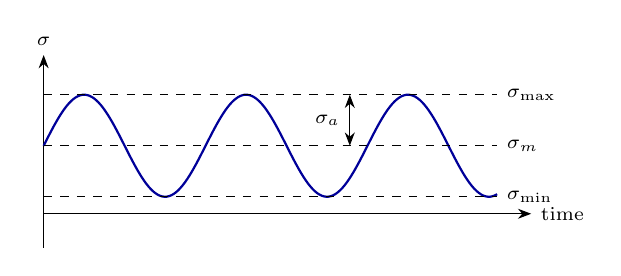
\begin{tikzpicture}[scale=0.72,>=Stealth,font=\scriptsize]
\draw[->] (0,0) -- (8.6,0) node[right] {time};
\draw[->] (0,-0.6) -- (0,2.8) node[above] {$\sigma$};
\draw[domain=0:8,samples=200,thick,blue!60!black] plot (\x,{1.2+0.9*sin(deg(\x*2.2))});
\draw[dashed] (0,1.2) -- (8,1.2) node[right] {$\sigma_m$};
\draw[dashed] (0,2.1) -- (8,2.1) node[right] {$\sigma_{\max}$};
\draw[dashed] (0,0.3) -- (8,0.3) node[right] {$\sigma_{\min}$};
\draw[<->] (5.4,1.2) -- (5.4,2.1) node[midway,left] {$\sigma_a$};
\end{tikzpicture}
\end{columns}
\vspace{4pt}
\begin{block}{}
Tensile mean stress is damaging; compressive mean stress is \emph{beneficial} --- which is why we shot-peen, cold-expand holes and use interference-fit fasteners.
\end{block}
\end{frame}


\begin{frame}{The same amplitude, three different mean stresses}
\centering

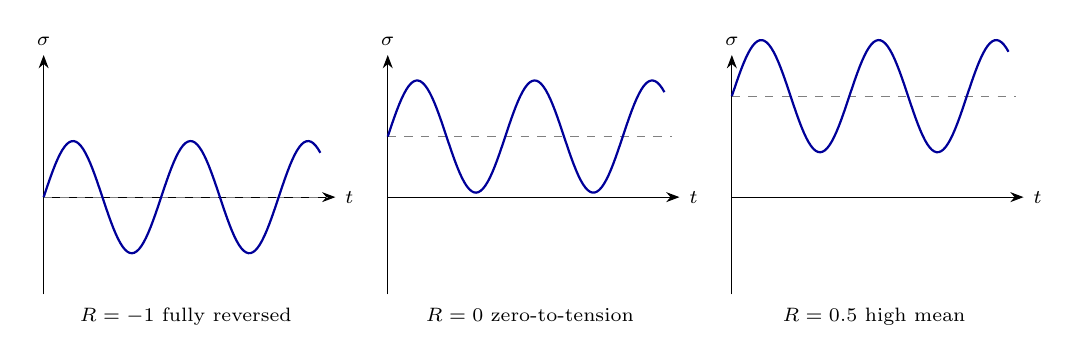
\begin{tikzpicture}[scale=0.95,>=Stealth,font=\scriptsize]
\foreach \i/\m/\lab in {0/0/{$R=-1$ fully reversed}, 1/0.9/{$R=0$ zero-to-tension}, 2/1.5/{$R=0.5$ high mean}} {
 \begin{scope}[xshift={\i*4.6cm}]
  \draw[->] (0,-1.3) -- (0,1.9) node[above] {$\sigma$};
  \draw[->] (0,0) -- (3.9,0) node[right] {$t$};
  \draw[dashed,gray] (0,{\m*0.9}) -- (3.8,{\m*0.9});
  \draw[domain=0:3.7,samples=120,thick,blue!60!black] plot (\x,{\m*0.9+0.75*sin(deg(\x*4))});
  \node[anchor=north,align=center] at (1.9,-1.35) {\lab};
 \end{scope}
}
\end{tikzpicture}

\vspace{6pt}
\footnotesize
All three have the same $\sigma_a$ --- and very different lives. Moving from $R=-1$ to $R=0.5$ at constant amplitude can cost an order of magnitude in cycles. This is what the mean-stress corrections later in the lecture are for.
\end{frame}

\section{Stress-life}

\begin{frame}{The S--N (Wöhler) curve and its three regions}
\centering

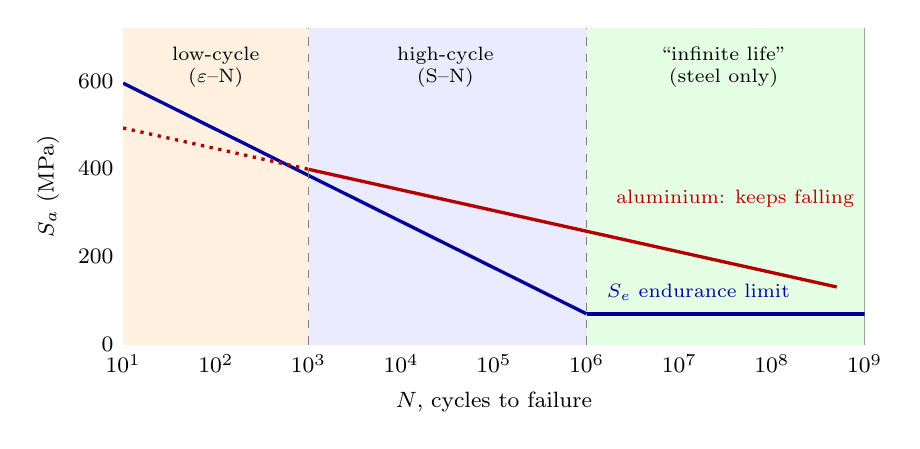
\begin{tikzpicture}
\begin{semilogxaxis}[width=11.0cm,height=5.6cm,xlabel={$N$, cycles to failure},ylabel={$S_a$ (MPa)},
 xmin=1e1,xmax=1e9,ymin=0,ymax=720,grid=both,grid style={gray!20},
 label style={font=\footnotesize},tick label style={font=\footnotesize}]
\fill[orange!12] (axis cs:1e1,0) rectangle (axis cs:1e3,720);
\fill[blue!8]   (axis cs:1e3,0) rectangle (axis cs:1e6,720);
\fill[green!10] (axis cs:1e6,0) rectangle (axis cs:1e9,720);
\addplot[very thick,blue!60!black,domain=1e3:1e6,samples=60]{700-105*log10(x)};
\addplot[very thick,blue!60!black,domain=1e6:1e9,samples=60]{70};
\addplot[very thick,blue!60!black,domain=1e1:1e3,samples=40]{700-105*log10(x)};
\addplot[very thick,red!70!black,domain=1e3:5e8,samples=100]{540-47*log10(x)};
\addplot[very thick,red!70!black,dotted,domain=1e1:1e3,samples=40]{540-47*log10(x)};
\node[font=\scriptsize,align=center,anchor=north] at (axis cs:1e2,700) {low-cycle\\ ($\varepsilon$--N)};
\node[font=\scriptsize,align=center,anchor=north] at (axis cs:3e4,700) {high-cycle\\ (S--N)};
\node[font=\scriptsize,align=center,anchor=north] at (axis cs:3e7,700) {``infinite life''\\ (steel only)};
\node[font=\scriptsize,anchor=south west,blue!60!black] at (axis cs:1.3e6,78) {$S_e$ endurance limit};
\node[font=\scriptsize,anchor=south,red!70!black] at (axis cs:4e7,290) {aluminium: keeps falling};
\draw[gray,dashed] (axis cs:1e3,0) -- (axis cs:1e3,720);
\draw[gray,dashed] (axis cs:1e6,0) -- (axis cs:1e6,720);
\end{semilogxaxis}
\end{tikzpicture}

\vspace{-2pt}
\begin{columns}[T]
\column{0.5\textwidth}\footnotesize
\begin{itemize}
  \item $N<10^3$: plasticity dominates $\Rightarrow$ use $\varepsilon$--N
  \item $10^3<N<10^6$: straight on log--log, $S_a=aN^{b}$
\end{itemize}
\column{0.5\textwidth}\footnotesize
\begin{itemize}
  \item Steel and titanium: a true limit $S_e$ at the knee --- below it, \alert{infinite life}
  \item \alert{Aluminium has no endurance limit}: quote a strength \emph{at a stated life} ($5\times10^{8}$)
\end{itemize}
\end{columns}
\end{frame}

\begin{frame}{First estimates --- and what you actually use}
\begin{columns}[T]
\column{0.5\textwidth}
Classical correlations:
\begin{align*}
S_e' &\approx 0.5\,S_{ut} \quad\text{(steel, } S_{ut}\le\SI{1400}{MPa})\\
S_e' &\approx \SI{700}{MPa} \quad\text{(steel above that)}\\
S_{f}&@5{\times}10^{8}\approx 0.4\,S_{ut}\ \text{(wrought Al)}\\
S_{1000}&\approx 0.9\,S_{ut}\ \text{bending},\ 0.75\,S_{ut}\ \text{axial}
\end{align*}
\[
b=-\tfrac13\log_{10}\!\frac{S_{1000}}{S_e},\quad a=\frac{S_{1000}}{(10^{3})^{b}}
\]
\column{0.5\textwidth}
\begin{alertblock}{Correlations are a sanity check, not an allowable}
For certification you use \alert{measured} data: MMPDS Ch.\ 9 gives S--N curves per alloy, product form, $K_t$ and $R$, fitted with the equivalent stress $S_{eq}=S_{\max}(1-R)^{p}$.
\end{alertblock}
\end{columns}
\end{frame}

\begin{frame}{From specimen to component: the Marin factors}
\[
S_e=k_a\,k_b\,k_c\,k_d\,k_e\,k_f\;S_e'
\]
\footnotesize
\begin{tabular}{@{}llp{7.4cm}@{}}
\toprule
$k_a$ & surface & $a\,S_{ut}^{b}$: ground (1.58, $-$0.085), machined (4.51, $-$0.265), hot-rolled (57.7, $-$0.718), forged (272, $-$0.995). As-forged on \SI{1200}{MPa} steel: $k_a\approx0.23$ \\
$k_b$ & size & $1.24\,d^{-0.107}$ ($d$ in mm); $k_b=1$ for axial. Bigger part $\Rightarrow$ more initiation sites \\
$k_c$ & loading & 1 bending, 0.85 axial, 0.59 torsion \\
$k_d$ & temperature & $\approx1$ to \SI{150}{\celsius} (Al), \SI{450}{\celsius} (steel) \\
$k_e$ & reliability & 0.897 (90\%), 0.868 (95\%), 0.814 (99\%), 0.753 (99.9\%) \\
$k_f$ & misc. & corrosion (\alert{removes the endurance limit entirely}), fretting ($3$--$10\times$), plating ($-10$ to $-35\%$), residual stress \\
\bottomrule
\end{tabular}
\vspace{2pt}
\normalsize
\begin{block}{}
Fatigue starts at the surface --- so the surface is where the designer's money goes.
\end{block}
\end{frame}

\begin{frame}{Notches: $K_t$ is not the whole story}
\[
K_f = 1+q\,(K_t-1),\qquad q=\frac{1}{1+\sqrt{a}/\sqrt{r}}
\]
\begin{columns}[T]
\column{0.52\textwidth}
\begin{itemize}
  \item Static ductile design ignores $K_t$; \alert{fatigue cannot}
  \item But the full $K_t$ is not realised either: a sharp notch has a steep gradient, so little material sees the peak
  \item $\sqrt{a}\approx0.25$--$\SI{0.5}{\sqrt{mm}}$ (high-strength steel), $\approx\SI{0.6}{\sqrt{mm}}$ (aluminium)
\end{itemize}
\column{0.48\textwidth}
\begin{alertblock}{The stronger the material, the more a notch punishes it}
$q\to1$ as strength rises. A \SI{1800}{MPa} 4340 part with a sharp fillet can be worse in fatigue than a \SI{900}{MPa} part with a generous one.
\end{alertblock}
\end{columns}
\vspace{2pt}
\footnotesize Apply $K_f$ to $\sigma_a$ (and conservatively to $\sigma_m$) --- \emph{or} divide $S_e$ by $K_f$. Never both.
\end{frame}

\begin{frame}{Mean stress: the constant-life diagram}
\begin{columns}[T]
\column{0.44\textwidth}
\footnotesize
\begin{align*}
\text{Goodman:}&\ \frac{\sigma_a}{S_e}+\frac{\sigma_m}{S_{ut}}=\frac1n\\
\text{Gerber:}&\ \frac{n\sigma_a}{S_e}+\Big(\frac{n\sigma_m}{S_{ut}}\Big)^{2}=1\\
\text{Soderberg:}&\ \frac{\sigma_a}{S_e}+\frac{\sigma_m}{S_{y}}=\frac1n\\
\text{Morrow:}&\ \frac{\sigma_a}{S_e}+\frac{\sigma_m}{\sigma_f'}=\frac1n
\end{align*}
\begin{itemize}
  \item Goodman: simple, conservative, \alert{the design standard}
  \item $\sigma_m<0$: take $\sigma_a=S_e$, claim no credit
  \item Always add the Langer yield check
\end{itemize}
\column{0.56\textwidth}
\centering
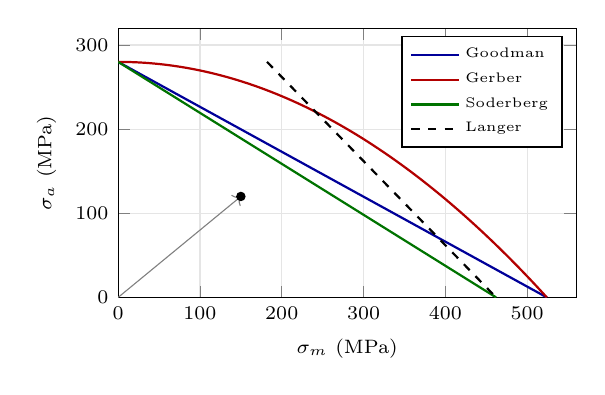
\begin{tikzpicture}
\begin{axis}[width=7.4cm,height=5.0cm,xlabel={$\sigma_m$ (MPa)},ylabel={$\sigma_a$ (MPa)},
  xmin=0,xmax=560,ymin=0,ymax=320,grid=both,grid style={gray!20},legend pos=north east,legend cell align=left,
  label style={font=\scriptsize},tick label style={font=\scriptsize},legend style={font=\tiny}]
\addplot[thick,blue!60!black,domain=0:524,samples=2]{280*(1-x/524)};
\addlegendentry{Goodman}
\addplot[thick,red!70!black,domain=0:524,samples=80]{280*(1-(x/524)^2)};
\addlegendentry{Gerber}
\addplot[thick,green!45!black,domain=0:462,samples=2]{280*(1-x/462)};
\addlegendentry{Soderberg}
\addplot[thick,black,dashed,domain=182:462,samples=2]{462-x};
\addlegendentry{Langer}
\addplot[only marks,mark=*,mark size=1.5pt,black] coordinates {(150,120)};
\draw[->,gray] (axis cs:0,0) -- (axis cs:150,120);
\end{axis}
\end{tikzpicture}
\end{columns}
\end{frame}

\begin{frame}{Variable amplitude: Palmgren--Miner}
\footnotesize
\[
D=\sum_i\frac{n_i}{N_i},\qquad \text{failure at } D=1
\]
\begin{columns}[T]
\column{0.5\textwidth}
\textbf{What it assumes --- and gets wrong}
\begin{itemize}
  \item Linear damage, no sequence effect
  \item Cycles below $S_e$ ignored
  \item Test data fail anywhere from $D=0.3$ to $3$
  \item High-low is worse than low-high
\end{itemize}
Haibach: keep a shallower slope below the knee rather than truncating.
\column{0.5\textwidth}
\textbf{Counting the cycles}
\begin{itemize}
  \item \alert{Rainflow} (ASTM E1049) --- the only method consistent with the material's hysteresis memory
  \item Level-crossing and peak counting are cruder ancestors
\end{itemize}
\textbf{Where the spectrum comes from}
\begin{itemize}\footnotesize
  \item GAG cycle (1/flight) --- usually dominant
  \item Pressurisation (1/flight), gust and manoeuvre exceedance curves, taxi, landing, braking
  \item Ordered flight-by-flight for test and analysis
\end{itemize}
\end{columns}
\end{frame}

\section{Worked examples}

\begin{frame}{Example 2.1 --- Machined 4340 shaft, 99\% reliability}
$S_{ut}=\SI{1240}{MPa}$, $d=\SI{30}{mm}$, machined, rotating bending
\begin{align*}
S_e' &= 0.5\times1240=\SI{620}{MPa}\\
k_a &= 4.51\times1240^{-0.265}=0.690,\qquad k_b=1.24\times30^{-0.107}=0.864\\
k_c &= 1,\quad k_d=1,\quad k_e=0.814\\
S_e &= 0.690\times0.864\times0.814\times620=\SI{297}{MPa}
\end{align*}
Add a fillet, $K_t=1.8$, $q=0.85$: $K_f=1.68$, so allowable $\sigma_a=297/1.68=\SI{177}{MPa}$.
\begin{alertblock}{48\% before the notch, 14\% of $S_{ut}$ after it}
A stronger steel would raise $S_{ut}$ but barely raise this number --- $k_a$ falls and $q$ rises with strength. A bigger fillet radius and a better finish would do far more.
\end{alertblock}
\end{frame}

\begin{frame}{Example 2.2 --- The fuselage lap joint}
2024-T3, $\sigma_\theta=\SI{75}{MPa}$ once per flight from zero $\Rightarrow \sigma_a=\sigma_m=\SI{37.5}{MPa}$, $R=0$.\\
Rivet hole: $K_t=3.0$, $q\approx0.9 \Rightarrow K_f=2.8$. Local $\sigma_a=\sigma_m=\SI{105}{MPa}$.
\[
\sigma_{a,\text{allow}}=140\left(1-\frac{105}{434}\right)=\SI{106}{MPa}
\qquad\text{(Goodman, }S_f@10^6=\SI{140}{MPa})
\]
\begin{itemize}
  \item Applied \SI{105}{MPa} sits \alert{on} the $10^{6}$-cycle line --- no margin for scatter
  \item A 60\,000-flight service goal would need a scatter factor of $\sim$17
  \item And this ignores secondary bending from the eccentric lap --- which can double it
\end{itemize}
\begin{block}{}
Hence the real answer: lower hoop stress, cold-expanded holes, bonded doublers --- or an explicit damage-tolerance justification with inspections.
\end{block}
\end{frame}

\begin{frame}{Example 2.3 --- Miner on a three-level spectrum}
Per flight: 1 GAG at \SI{120}{MPa}, 10 manoeuvre at \SI{80}{MPa}, 200 gust at \SI{40}{MPa}; $S_a=1100N^{-0.13}$
\vspace{2pt}
\centering\footnotesize
\begin{tabular}{@{}lrrrr@{}}
\toprule
Level & $\sigma_a$ (MPa) & $n$/flight & $N$ & $n/N$ \\
\midrule
GAG & 120 & 1 & $2.5\times10^{7}$ & $4.0\times10^{-8}$ \ (67\%) \\
Manoeuvre & 80 & 10 & $5.7\times10^{8}$ & $1.8\times10^{-8}$ \ (30\%) \\
Gust & 40 & 200 & $1.2\times10^{11}$ & $1.7\times10^{-9}$ \ (3\%) \\
\midrule
& & & $D$/flight & $5.9\times10^{-8}$ \\
\bottomrule
\end{tabular}
\vspace{4pt}

\raggedright\normalsize Life $=1.7\times10^{7}$ flights; with a scatter factor of 4, $4.2\times10^{6}$ certified.
\begin{alertblock}{The pattern is general}
The one big cycle does two-thirds of the damage; 200 small ones do 3\%. Reduce the \emph{peaks}. Truncating the low end barely matters --- truncating the high end is a serious error.
\end{alertblock}
\end{frame}

\section{Strain-life}

\begin{frame}{Why S--N runs out}
\begin{itemize}
  \item At a notch root under a large load the local material \alert{yields} even though the nominal stress is elastic
  \item Stress then no longer characterises the loading: the notch root is \emph{strain-controlled} by the elastic material around it
  \item Needed for $N<10^{4}$, for notches in ductile alloys, and for thermal or displacement-controlled loading
  \item It is also the physically correct description of crack \emph{initiation}, and the basis of modern fatigue software
\end{itemize}
\begin{block}{Cyclic stress--strain}
Metals cyclically harden or soften to a stable hysteresis loop:
$\dfrac{\Delta\varepsilon}{2}=\dfrac{\Delta\sigma}{2E}+\Big(\dfrac{\Delta\sigma}{2K'}\Big)^{1/n'}$, with $n'\approx0.1$--$0.2$.
\end{block}
\end{frame}

\begin{frame}{Coffin--Manson--Basquin}
\begin{columns}[T]
\column{0.42\textwidth}
\[
\frac{\Delta\varepsilon}{2}=\frac{\sigma_f'}{E}(2N_f)^{b}+\varepsilon_f'(2N_f)^{c}
\]
\footnotesize
\begin{itemize}
  \item $b\approx-0.05$ to $-0.12$ (strength)
  \item $c\approx-0.5$ to $-0.7$ (ductility)
  \item $2N_f$ = reversals, not cycles
\end{itemize}
\begin{alertblock}{The design dilemma, in one plot}
Below $N_t$: \alert{ductility} wins --- a tough alloy outlives a strong one. Above $N_t$: \alert{strength} wins.
\end{alertblock}
\column{0.58\textwidth}
\centering
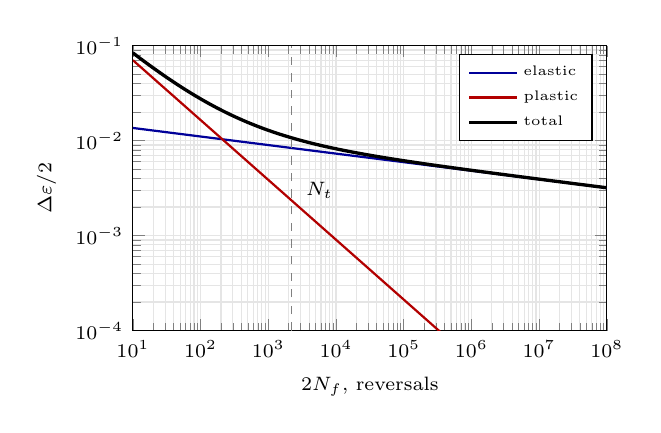
\begin{tikzpicture}
\begin{loglogaxis}[width=7.6cm,height=5.2cm,xlabel={$2N_f$, reversals},ylabel={$\Delta\varepsilon/2$},
  xmin=1e1,xmax=1e8,ymin=1e-4,ymax=1e-1,grid=both,grid style={gray!20},legend pos=north east,legend cell align=left,
  label style={font=\scriptsize},tick label style={font=\scriptsize},legend style={font=\tiny}]
\addplot[thick,blue!60!black,domain=1e1:1e8,samples=80]{(1200/71700)*x^(-0.09)};
\addlegendentry{elastic}
\addplot[thick,red!70!black,domain=1e1:1e8,samples=80]{0.3*x^(-0.63)};
\addlegendentry{plastic}
\addplot[very thick,black,domain=1e1:1e8,samples=120]{(1200/71700)*x^(-0.09)+0.3*x^(-0.63)};
\addlegendentry{total}
\draw[gray,dashed] (axis cs:2.2e3,1e-4) -- (axis cs:2.2e3,1e-1);
\node[font=\scriptsize,anchor=west] at (axis cs:2.6e3,3e-3) {$N_t$};
\end{loglogaxis}
\end{tikzpicture}
\end{columns}
\end{frame}

\begin{frame}{Neuber's rule --- getting local from nominal}
\footnotesize
\[
K_f^{2}=K_\sigma K_\varepsilon \quad\Longrightarrow\quad \sigma\varepsilon=\frac{(K_f S)^{2}}{E}
\]
Solve this hyperbola \emph{simultaneously} with the cyclic stress--strain curve; the resulting $\varepsilon_a$ goes into Coffin--Manson.
\vspace{4pt}
\begin{columns}[T]
\column{0.52\textwidth}
\textbf{Example 2.4} --- 7075-T6, hole with $K_f=2.6$, nominal $S_a=\SI{150}{MPa}$ (29\% of $S_{ut}$)
\begin{align*}
\sigma\varepsilon&=(2.6\times150)^2/71\,700=\SI{2.12}{MPa}\\
\Rightarrow\ \sigma&\approx\SI{379}{MPa},\quad \varepsilon\approx5.59\times10^{-3}\\
\text{(elastic)}\ &\ \sigma=390,\ \varepsilon=5.44\times10^{-3}\\
\Rightarrow\ 2N_f&\approx2.5\times10^{5},\quad N_f\approx1.2\times10^{5}
\end{align*}
\column{0.48\textwidth}
\begin{block}{Two remarks}
\begin{itemize}
  \item The notch root yields on cycle 1 at less than a third of $S_{ut}$ nominal --- normal at a fastener hole
  \item This is life to \alert{initiation} of a small crack. What remains is a crack-growth problem
\end{itemize}
\end{block}
\scriptsize Glinka's energy rule is less conservative; mean stress enters via Morrow or SWT.
\end{columns}
\end{frame}

\section{Fatigue in the certification codes}

\begin{frame}{CS-25.571: three philosophies}
\footnotesize
\begin{itemize}
  \item \alert{Safe-life} --- retire the part at (demonstrated life)/(scatter factor $\approx$ 3--5). No cracks assumed. Landing gear, engine discs, some rotorcraft parts
  \item \alert{Fail-safe} --- a second load path carries limit load after any single failure. (The dual-lug fix from last lecture's error gallery)
  \item \alert{Damage tolerance} --- cracks are assumed to exist; inspections are scheduled to find them before they are critical. The default for transport metallic structure, and next lecture's subject
\end{itemize}
\begin{block}{Where the scatter factor comes from}
Every approximation in this lecture: S--N scatter, Miner's non-linearity, uncertainty in $K_f$, surface and environment, and the variability of the usage spectrum.
\end{block}
\vspace{2pt}
\footnotesize \href{https://www.easa.europa.eu/en/document-library/easy-access-rules/online-publications/easy-access-rules-large-aeroplanes-cs-25}{CS-25.571 and AMC 25.571 (EASA Easy Access Rules)} \ $\cdot$ \ FAA AC 25.571-1D
\end{frame}

\begin{frame}{Design levers, in order of effectiveness}
\begin{enumerate}
  \item \alert{Remove the stress concentration}: larger radii, gentler transitions
  \item \alert{Reduce the peak cycles} --- they dominate the damage sum
  \item \alert{Improve the surface}: finish, shot peening, cold-expanded holes, interference fasteners (cold expansion alone buys $3$--$5\times$ life --- the biggest single gain available)
  \item Introduce compressive residual stress; avoid tensile mean stress
  \item Protect from corrosion and fretting; specify plating and sealing
  \item \emph{Only then}: change the material or add thickness
\end{enumerate}
\begin{alertblock}{}
Adding thickness is the last resort, not the first. It adds weight, and it does nothing about a sharp corner.
\end{alertblock}
\end{frame}

\section{For next time}

\begin{frame}{For next time}
\begin{itemize}
  \item Shigley Ch.\ 6, \S\S6.1--6.17; Dowling Ch.\ 9--10 and 14
  \item MMPDS Ch.\ 9: look up the S--N curves for 2024-T3 and 7075-T6 at $K_t=1$ and $K_t=3$ and compare
  \item Read \href{https://www.easa.europa.eu/en/document-library/easy-access-rules/online-publications/easy-access-rules-large-aeroplanes-cs-25}{CS-25.571} with its AMC
  \item Self-study problems 1--6 in the notes (two are Python: an $\varepsilon$--N solver and rainflow counting)
  \item Next: fracture mechanics --- what happens \emph{after} the crack exists, and how damage tolerance sets inspection intervals
\end{itemize}
\end{frame}

\end{document}
